\documentclass[a4paper]{article}
\usepackage{amsfonts}
\usepackage{amsmath}
\usepackage{amssymb}
\usepackage{graphicx}     

\begin{document}
  
\noindent \large Auteur: Rubin Cuypers \\
\noindent \large Studierichting: Informatica\\
\noindent \large Oefeningenreeks 5G nr. 1.11\\

\medskip

\normalsize

$f(x)=\tan x$,  $x \in \left[0,\dfrac{\pi}{4}\right]$\\

$V=\pi \displaystyle \int_{0}^{\dfrac{\pi}{4}} \tan^2 x dx$\\

$=\pi \displaystyle \int_{0}^{\dfrac{\pi}{4}} \left(\sec^2 x -1\right) dx$\\

$=\pi \left[\tan x - x \right]_0^{\dfrac{\pi}{4}} = \pi \left( \tan \dfrac{\pi}{4} - \dfrac{\pi}{4} \right) $\\

$ =\pi \left( 1- \dfrac{\pi}{4} \right)$\\



\begin{figure}[h]
    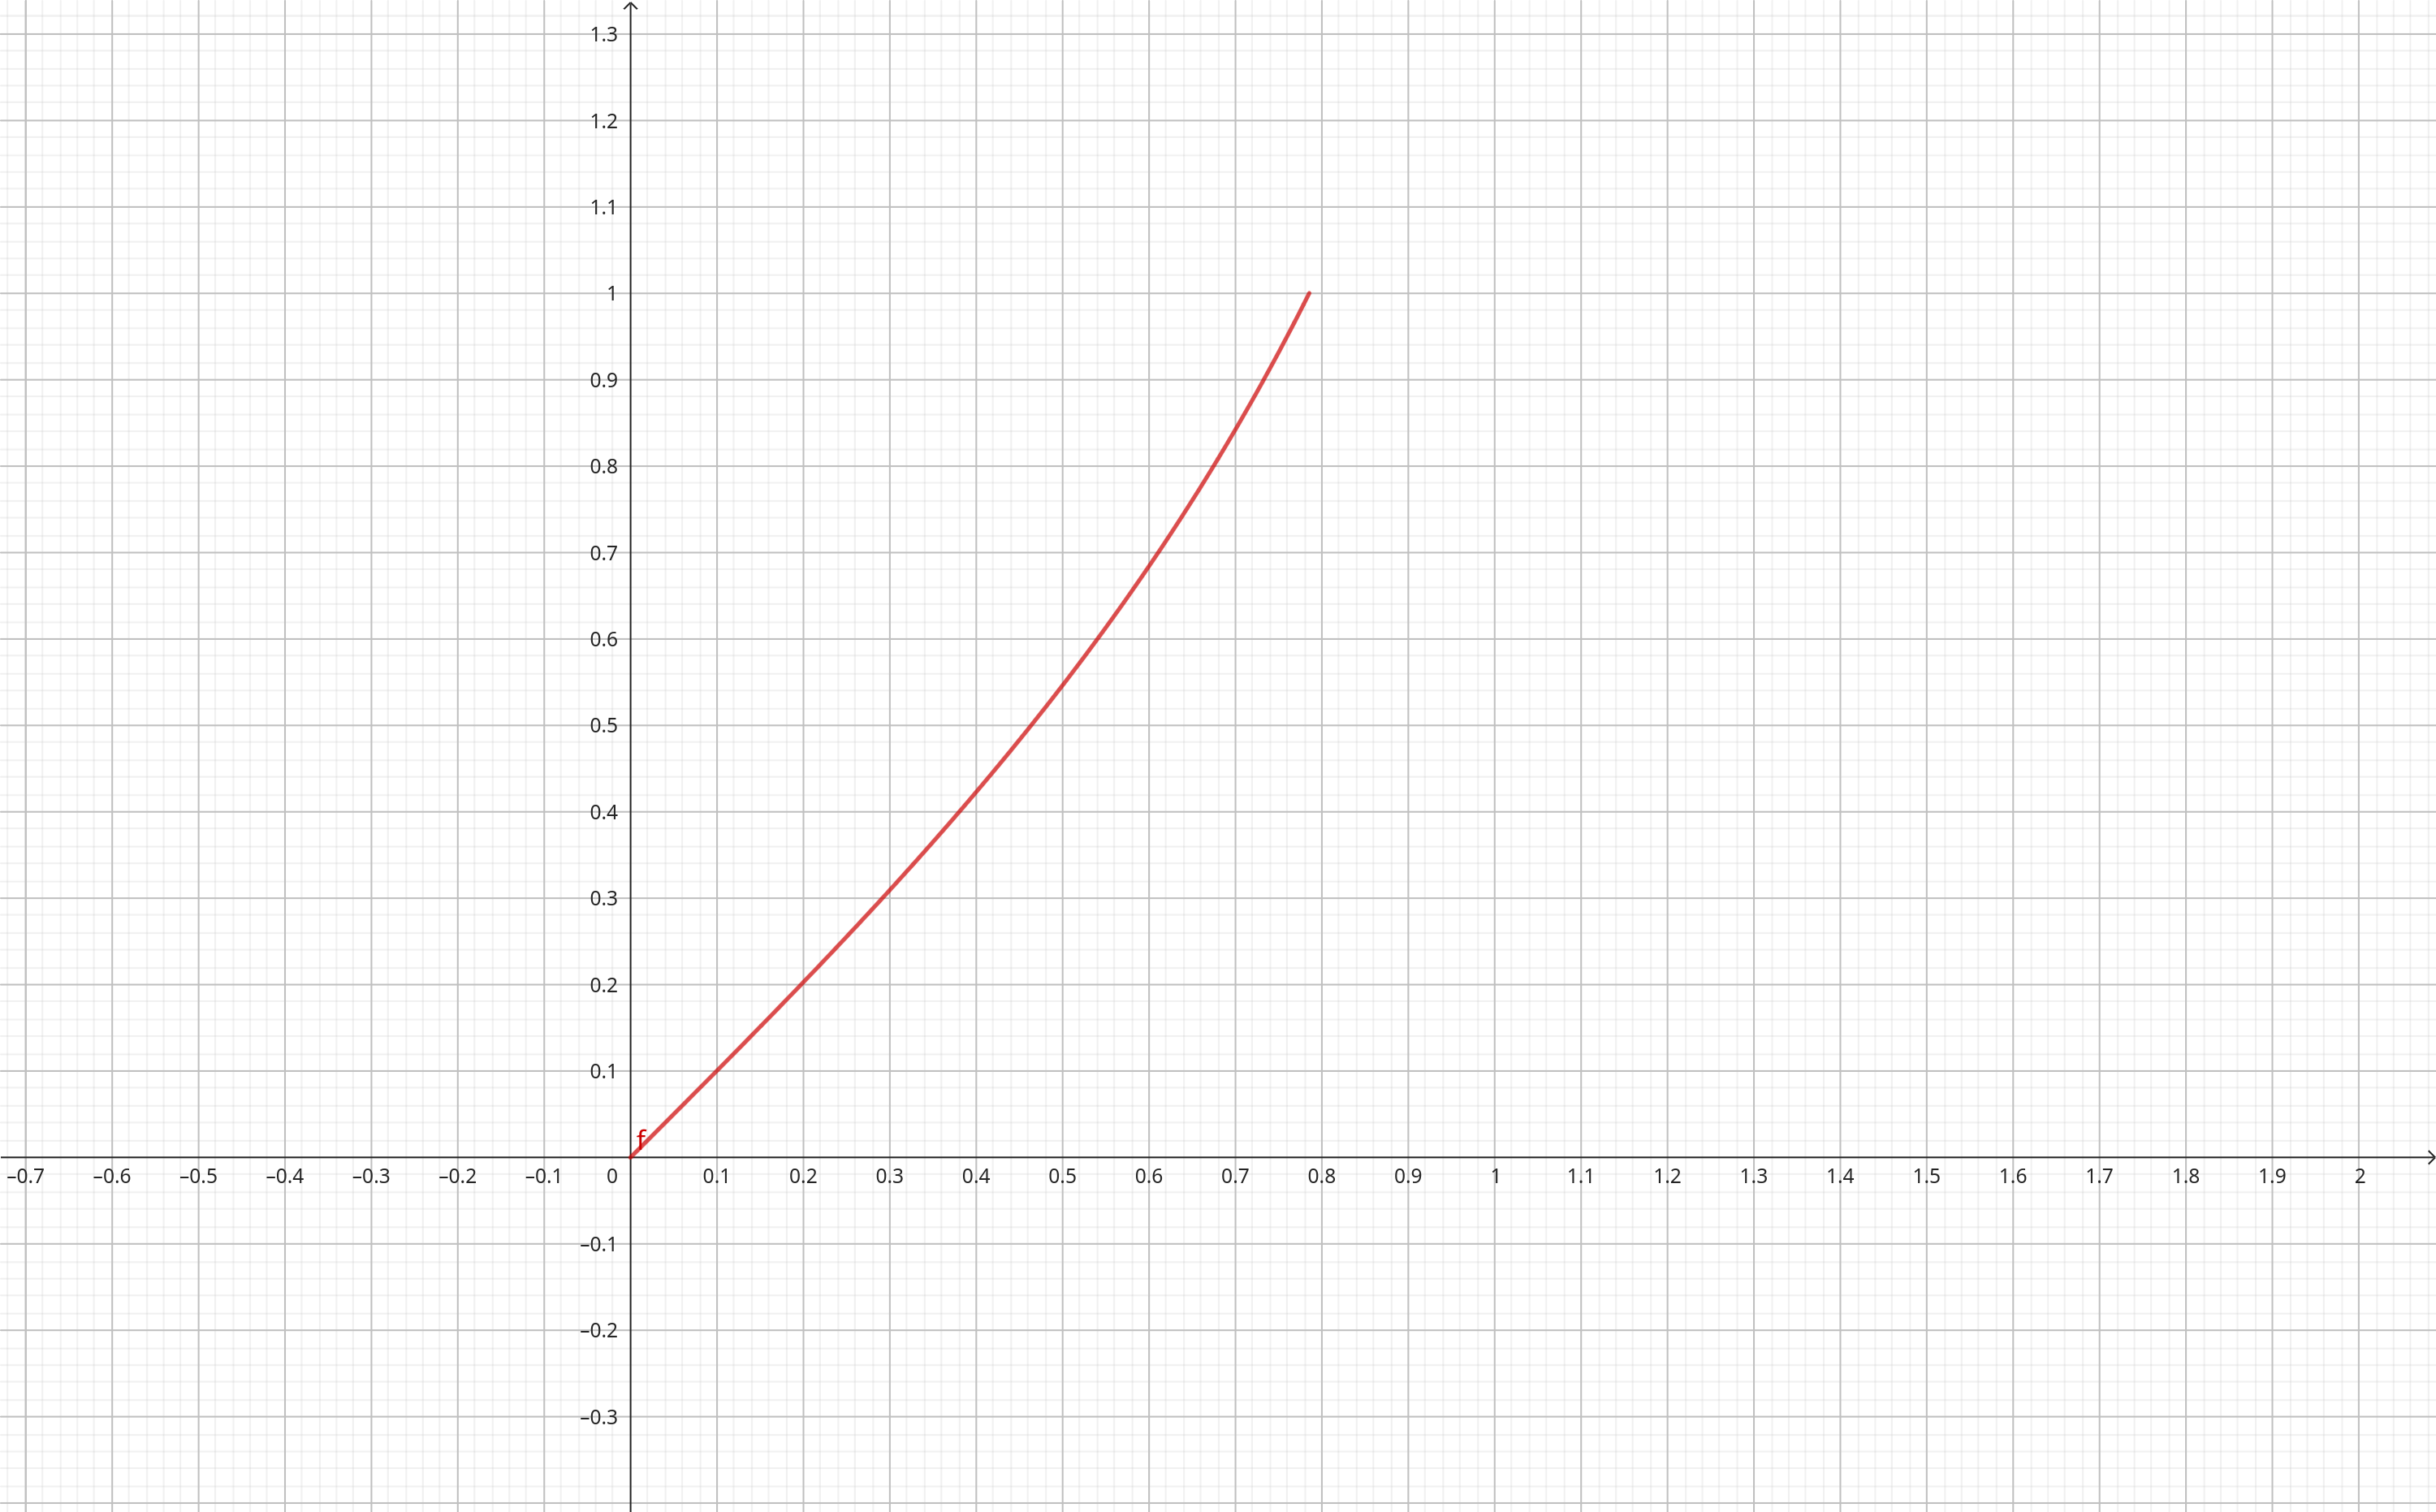
\includegraphics[width=\linewidth]{5G-1.11-rubin.cuypers.INF.png}\\
\end{figure}

\begin{thebibliography}{999}
%\bibitem{a} Referentie
\end{thebibliography}
\end{document} 
